%!TEX encoding = UTF-8 Unicode
\documentclass[12pt]{book}          %Abschlußarbeit 12pt-book
\usepackage[utf8]{inputenc}         %empfohlene Zeichenkodierung UTF-8
\usepackage[T1]{fontenc}            %empfohlene Fontkodierung
\usepackage{lmodern}                %besserer Font
\usepackage{microtype}              %bessere Zeichenabstände
\usepackage[german]{babel}          %deutsch
\usepackage{hyperref}               % um auf sections zu verweisen
\usepackage{csquotes}               % Required for fine quoting
\usepackage{enumitem}               % Required for nested arabic Enumeration
\usepackage{graphicx}               % Required for inserting images
\usepackage[Algorithmus]{algorithm} % Algorithmen
\usepackage{algpseudocode}
\usepackage{listings}
\usepackage{chngcntr}
\algnewcommand\algorithmicforeach{\textbf{for each}}
\algdef{S}[FOR]{ForEach}[1]{\algorithmicforeach\ #1\ \algorithmicdo}
\usepackage[
backend=biber,
style=alphabetic
]{biblatex}                         %required for citations
\usepackage[
    a4paper,
    margin=2.5cm
]{geometry}                         %Seitenmaße
\parskip.5\baselineskip

%Algorithmen
\lstdefinelanguage{JavaScript}{
  keywords={break, case, catch, continue, debugger, default, delete, do, else, finally, for, function, if, in, instanceof, new, return, switch, this, throw, try, typeof, var, void, while, with, export, interface, string, boolean, const, false, true},
  morecomment=[l]{//},
  morecomment=[s]{/*}{*/},
  morestring=[b]",
  morestring=[b]'
}
\lstset{language=JavaScript, basicstyle=\ttfamily, keywordstyle=\bfseries, showstringspaces=false}
\renewcommand{\listalgorithmname}{Algorithmenverzeichnis}
\counterwithin{algorithm}{chapter}




\addbibresource{bibliography.bib} %Imports bibliography file


%--------------TITEL-----------------
%------------------------------------
\title{
\begin{center}
   \parskip1\baselineskip

   \large
   Abschlussarbeit am LG Kooperative Systeme der FernUniversität in Hagen
   
   ~
   
   \LARGE\bfseries 
    YReduxSocket: Ein Werkzeug zur Synchronisation und Konsistenz in Webanwendungen

   \large
   Ricardo Stolzlechner
   
   9463470
   
   ricardo.stolzlechner@gmail.com
   
   Informatik Bachelor of Science
   
   Betreuerin: Dr. Lihong Ma
\end{center}
}

\author{}

\begin{document}

\maketitle

%--------------ABSTRACT-------------------
%-----------------------------------------
\chapter*{Abstract}

\newpage

%--------------VERZEICHNISSE--------------
%-----------------------------------------
\tableofcontents
%\listoftables %uncomment this if more than one table is used
\listoffigures
\listofalgorithms

\newpage

%--------------EINLEITUNG--------------
%--------------------------------------
\chapter{Einleitung}
\label{chap-einleitung}

\section{Hintergrund und Motivation}
\label{sec-hintergrund-und-motivation}

Die Webanwendung "`Yoshie.io"'\footnote{https://www.yoshie.io/} ist eine kollaborative Plattform, spezialisiert auf das Baugewerbe. Der Autor dieser Arbeit fungiert hier als technischer Leiter. Im Baugewerbe operieren die verschiedenen Gewerke häufig in isolierten Datensilos. Baupläne und ähnliche Dokumente liegen bei den Beteiligten in unterschiedlichen Versionen vor, was während der Bauphase oft zu Fehlern und damit verbundenen Mehrkosten führt. "`Yoshie.io"' bietet eine Lösung, indem es eine Plattform zur Verfügung stellt, auf der sämtliche für ein Bauvorhaben erforderlichen Dokumente zentralisiert, versioniert und zugänglich gemacht werden. 

Während der Entwicklung dieser Anwendung wurde offensichtlich, dass eine der zentralen Herausforderungen darin besteht, die Konsistenz der dargestellten Daten zu gewährleisten. Diese Anforderung lässt sich in zwei Hauptbereiche unterteilen, die unterschiedliche technologische Ansätze erfordern. Einerseits muss die Datenkonsistenz innerhalb der verschiedenen Komponenten desselben Clients sichergestellt werden. Andererseits ist es notwendig, Datenänderungen zwischen verschiedenen Clients zu synchronisieren. Basierend auf Tanenbaum und van Steen musste ein clientbasiertes Konsistenzmodell implementiert werden, welches die Eigenschaften \textit{monotones Lesen}, \textit{monotones Schreiben} sowie eine \textit{Writes Follow Reads} Konsistenz aufweist \cite[322-325]{tanenbaum_verteilte_2008}. In diesem Zusammenhang wurden ein auf Redux basierender Datenstore und das WebSocket-Kommunikationsprotokoll als technologische Lösungen eingesetzt.

Der Aufwand für die Implementierung und Wartung der Anwendung im Bereich der Konsistenzerhaltung stieg zunehmend. Daher wurde ein Konzept entwickelt, das beide Technologien kombiniert, um so den Entwicklungsaufwand erheblich zu reduzieren. Dieses Konzept erhielt intern den Namen \textit{YReduxSocket}. Im Rahmen dieser Arbeit soll das genannte Konzept detailliert betrachtet und spezifiziert werden.

\section{Problemstellung}
\label{sec-problemstellung}

Wie bereits in Abschnitt \ref{sec-hintergrund-und-motivation} erwähnt, ergeben sich im Kontext der Konsistenzerhaltung in Webanwendungen zwei unterschiedliche Problemfelder. Diese werden in den folgenden Abschnitten näher erläutert.

\subsection{Datenkonsistenz am selben Client}
\label{subsec-datenkonsistenz-am-selben-client}

JavaScript-Frameworks wie \textit{React} oder \textit{Angular} basieren auf einer komponentenorientierten Architektur. Hierbei, stellt jede Komponente ein User-Interface-Element dar, das an verschiedenen Stellen innerhalb der Anwendung eingesetzt werden kann. Diese Komponenten können weitere Unterkomponenten umfassen, wodurch ein Komponentenbaum entsteht. Typischerweise gibt es in Webanwendungen zahlreiche verschiedene Komponenten,
deren Daten im Baum ausgetauscht und synchronisiert werden müssen.

Häufig sollen verschiedene Komponenten identische Daten anzeigen. In solchen Fällen ist es die Aufgabe der Entwicklerin, sicherzustellen, dass die Daten zwischen diesen Komponenten synchronisiert bleiben. Aufgrund der Notwendigkeit einer losen Kopplung, bei der Unterkomponenten keine direkte Kenntnis von ihren Elternkomponenten haben, ist die Synchronisation dieser Daten keine triviale Aufgabe.

\begin{figure}[htbp]
\centering
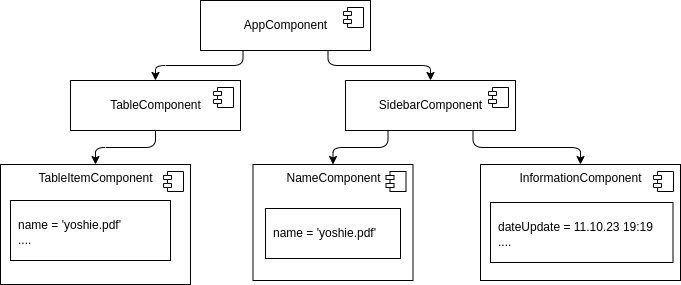
\includegraphics[height=6cm]{abbildungen/components-sync-1.png}
\caption{UML-Diagramm eines einfachen Komponentenbaums}
\label{simple-component-tree-uml}
\end{figure}

\begin{figure}[htbp]
\centering
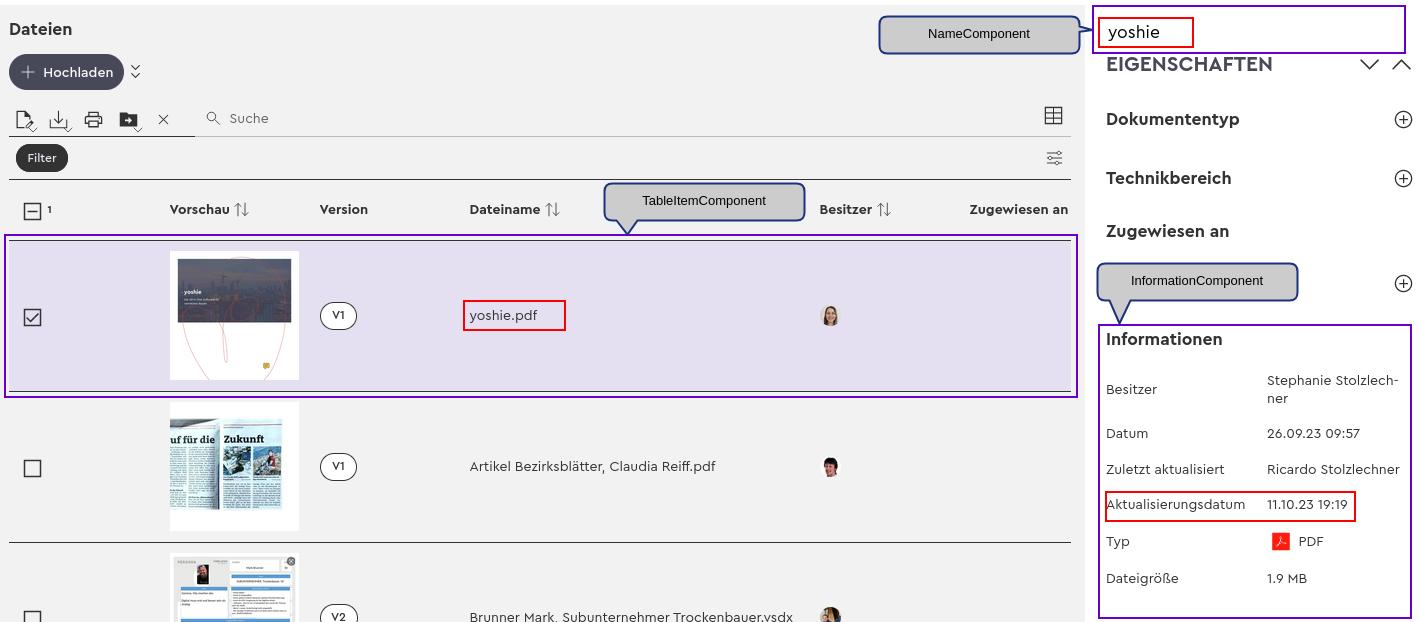
\includegraphics[height=7cm]{abbildungen/simple-comp-tree-screenshot.png}
\caption{Bildschirmausschnitt eines einfachen Komponentenbaums}
\label{simple-component-tree-screenshot}
\end{figure}

In Abbildung \ref{simple-component-tree-uml} wird ein einfacher Komponentenbaum gezeigt. Der zugehörige Bildschirmausschnitt dieses Baums ist in Abbildung \ref{simple-component-tree-screenshot} zu sehen. Die Komponenten \texttt{TableItemComponent} und \texttt{NameComponent} zeigen jeweils dasselbe Datenfeld an. Wird der Name in der \texttt{NameComponent} geändert, muss der Entwickler dafür sorgen, dass diese Information auch an die \texttt{TableItemComponent} weitergegeben wird. Zudem muss das Aktualisierungsdatum in der \texttt{InformationComponent} aktualisiert werden.

Verschiedene Ansätze, um die notwendige Synchronisierung zu erreichen, werden in späteren Kapiteln detailliert betrachtet und miteinander verglichen.

\subsection{Datenkonsistenz zwischen verschiedenen Clients}
\label{subsec-datenkonsistenz-zwischen-zwei-verschiedenen-clients}

In einer Webanwendung arbeiten verschiedene Clients oft mit denselben Daten. Wenn beispielsweise zwei Benutzerinnen gleichzeitig dieselbe Ansicht, wie in Abbildung \ref{simple-component-tree-screenshot} dargestellt, geladen haben und eine von ihnen den Namen über die \texttt{NameComponent} ändert, muss gewährleistet sein, dass diese Änderung auch bei der anderen Benutzerin sichtbar wird. Daher ist es erforderlich, einen Mechanismus zu etablieren, der bei Datenänderungen alle betroffenen Teilnehmer synchron hält. Verschiedene Ansätze zur Lösung dieses Problems werden in späteren Abschnitten vorgestellt.


\section{Ziele der Arbeit}
\label{sec-ziele-der-arbeit}

Wie bereits erwähnt, existieren diverse Ansätze zur Lösung der beiden beschriebenen Probleme. Das Konzept \textit{YReduxSocket} zielt darauf ab, beide Konsistenzanforderungen zu vereinheitlichen und gemeinsam zu adressieren. Hierbei wird auf jedem Client ein eigner auf Redux basierender Datenstore verwendet. Diese Datenstores werden anschließend mithilfe des WebSocket-Kommunikationsprotokolls, welches von einer zentralen Serverinstanz gesteuert wird, synchronisiert. Ein besonderer Fokus bei der Entwicklung von \textit{YReduxSocket} lag auf der Entwicklerfreundlichkeit. Das Konzept minimiert die bei Funktionserweiterungen notwendigen Änderungen bezüglich des Konsistenzverhaltens. Dies trägt zur Reduzierung von Entwicklungsfehlern bei und verbessert somit das Konsistenzverhalten von Webanwendungen.

Das primäre Ziel dieser Arbeit besteht darin, \textit{YReduxSocket} und die zugrundeliegenden Technologien generisch zu spezifizieren. Ein besonderes Augenmerk liegt auf der detaillierten Untersuchung des Konsistenzverhaltens des Konzepts. Weiterhin ist geplant, \textit{YReduxSocket} mit anderen Ansätzen zu vergleichen, um Verbesserungspotenziale zu identifizieren und gegebenenfalls zu implementieren. Zusätzlich wird die vorgestellte Spezifikation in verschiedenen Frameworks implementiert, um deren praktische Anwendbarkeit zu testen. \\

\section{Struktur der Arbeit}
\label{sec-struktur-der-arbeit}

Zu Beginn werden in Kapitel \ref{chap-grundlagen} die grundlegenden Konzepte erörtert, die für das Verständnis der weiteren Arbeit essenziell sind. Dabei liegt der Fokus auf Single Page Applications, der komponentenbasierten Webentwicklung, dem zentralen Redux-basierten Datenstore sowie dem WebSocket-Kommunikationsprotokoll. Ferner wird definiert, welche Voraussetzungen für den Einsatz von \textit{YReduxSocket} erfüllt sein müssen. Im abschließenden Teil dieses Kapitels wird ein Ansatz vorgestellt, wie ein Datenstore mittels WebSocket-Nachrichten synchronisiert werden kann.

Im anschließenden Kapitel \ref{chap-stand-der-technik} werden verwandte Arbeiten und Konzepte, die im Zuge einer Literaturrecherche sowie auf Open-Source-Plattformen identifiziert wurden, detailliert analysiert.

Kapitel \ref{chap-y-redux-socket} ist dem Konzept \textit{YReduxSocket} gewidmet. Hier wird das Konzept zunächst generisch vorgestellt und spezifiziert. Der Abschnitt \ref{sec-konsistenzverhalten} vertieft das Thema, indem das Konsistenzverhalten von \textit{YReduxSocket} genauer beleuchtet wird. Das Kapitel schließt mit einem Vergleich von \textit{YReduxSocket} mit den in Abschnitt \ref{sec-datenstore-mit-websocket-herkoemmlicher-ansatz} und Kapitel \ref{chap-stand-der-technik} vorgestellten Ansätzen.

In Kapitel \ref{chap-implementierung-und-tests} werden verschiedene Implementierungen von \textit{YReduxSocket} behandelt. Abschnitt \ref{sec-angular-und-aps-net} erläutert den Einsatz von \textit{YReduxSocket} in Verbindung mit den Frameworks \textit{Angular} und \textit{ASP.NET}, während Abschnitt \ref{sec-react-und-node-js} die Anwendung in den Frameworks \textit{React} und \textit{Node.js} beschreibt. Das Kapitel endet mit einer Darstellung, wie \textit{YReduxSocket} in gängigen Paketplattformen, konkret \textit{npm} und \textit{NuGet}, integriert werden kann.

Die Arbeit wird mit Kapitel \ref{chap-fazit} abgerundet. In diesem Abschnitt werden die erzielten Ergebnisse zusammengefasst, die Lösung validiert und potenzielle Verbesserungen des Konzepts aufgezeigt. 



%--------------GRUNDLAGEN--------------
%--------------------------------------
\chapter{Grundlagen}
\label{chap-grundlagen}

In diesem Kapitel werden grundlegende Konzepte vorgestellt, die eine solide Basis für das Verständnis des weiteren Inhalts dieser Arbeit bilden. Es werden außerdem jene Voraussetzungen definiert, die für den erfolgreichen Einsatz von \textit{YReduxSocket} notwendig sind.

\section{Single Page Applications (SPAs)}
\label{sec-single-page-applications}

Single Page Applications (SPAs) zeichnen sich dadurch aus, dass die gesamte Anwendung im Webbrowser des Benutzers ausgeführt wird. Eine SPA wird von einem Webserver bereitgestellt, der eine \texttt{index.html} Datei enthält. Diese wird ausgeliefert, sobald die entsprechende URL im Webbrowser aufgerufen wird. In der \texttt{index.html} befindet sich ein \texttt{script}-Tag, das auf den erforderlichen JavaScript-Code für die Ausführung der Anwendung verweist. Dieser Code wird vom Browser heruntergeladen und ausgeführt. Nach dem initialen Ladevorgang beschränkt sich die Rolle des Webservers darauf, statische Ressourcen wie Schriftarten oder Bilder nachzuladen. Die benötigten HTML-Elemente für die Darstellung werden ausschließlich über JavaScript generiert und aktualisiert. Für die Entwicklung von SPAs werden verschiedene etablierte Frameworks wie \textit{Angular}, \textit{React} und \textit{Vue} verwendet, die die DOM-API des Webbrowsers abstrahieren und somit die Entwicklung vereinfachen. Dies steht im Gegensatz zu klassischen Webanwendungen, bei denen der HTML-Code serverseitig generiert und ausgeliefert wird, bekannt als serverseitiges Rendering \cite[1]{hartmann_react_2020}.

\begin{figure}[htbp]
\centering
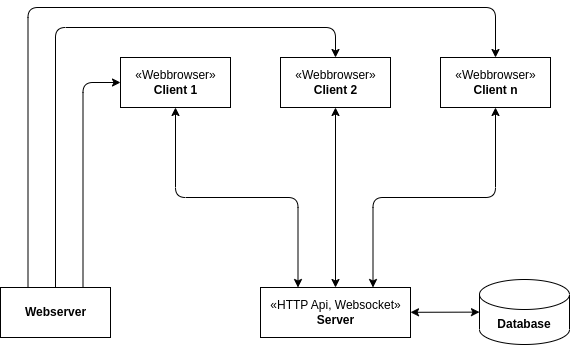
\includegraphics[height=7cm]{abbildungen/spa-architecture.png}
\caption{Von \textit{YReduxSocket} vorausgesetzte Prozessarchitektur}
\label{spa-architecture}
\end{figure}

\textit{YReduxSocket} setzt den Einsatz einer Single Page Application voraus. Zusätzlich wird eine separate Serverinstanz benötigt, die von den Clients zum Abrufen und Bearbeiten von Datensätzen verwendet wird. Diese Serverinstanz bietet eine HTTP-API und ermöglicht die Einrichtung einer WebSocket-Kommunikation. Jegliche Kommunikation zwischen den Clients läuft über diese Serverinstanz, die als eigenständiger Prozess zu verstehen ist und nicht mit dem Webserver, der die SPA bereitstellt, verwechselt werden sollte. Im weiteren Verlauf der Arbeit bezieht sich der Begriff "`Server"' stets auf diese separate Serverinstanz. Die in Abbildung \ref{spa-architecture} dargestellte Struktur illustriert die von \textit{YReduxSocket} benötigte Prozessarchitektur, wobei jedes Rechteck im Diagramm einen unabhängigen Prozess repräsentiert.

\section{Komponentenbasierte Webentwicklung}
\label{sec-komponentenbasierte-webentwicklung}

Wie im Abschnitt \ref{sec-single-page-applications} erwähnt, erleichtern Frameworks den Aufbau von Single Page Applications (SPAs), indem sie auf einer komponentenbasierten Architektur aufbauen. Eine Komponente gliedert sich grundsätzlich in zwei Teile: Der erste Teil, in einer Art HTML definiert, beschreibt die Darstellung der Komponente im Browser. Der zweite Teil, mit JavaScript oder TypeScript (einer typisierten Variante von JavaScript) formuliert, definiert die logische Funktionalität der Komponente, einschließlich Methoden für Nutzerinteraktionen.

Jede Komponente kann im HTML-Teil weitere Unterkomponenten beinhalten, wodurch ein Komponentenbaum gebildet wird. Die Komponenten stehen so in einer Eltern-Kind-Beziehung zueinander.

In Webanwendungen müssen viele Komponenten miteinander kommunizieren. Dafür stellen Frameworks verschiedene Datenbindungsmechanismen zur Verfügung. Eine Eltern-Komponente kann Daten über einen Eingabeparameter an eine Kind-Komponente übergeben. Kind-Komponenten können Ausgabeparameter bereitstellen, über die sie die Eltern-Komponenten bezüglich Datenänderungen informieren. Wenn Kind-Komponenten diese Ausgabeparameter aktualisieren, wird die Eltern-Komponente automatisch benachrichtigt, sofern sie sich auf diese registriert hat.

\begin{figure}[htbp]
\centering
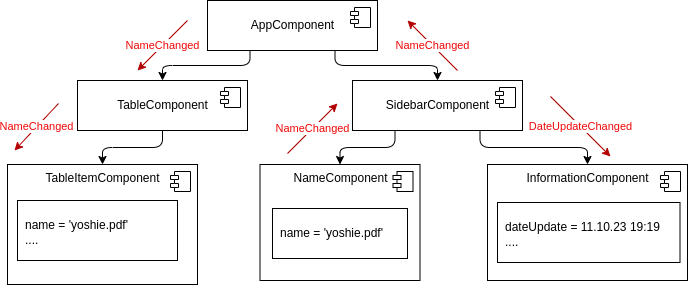
\includegraphics[height=6.5cm]{abbildungen/components-sync-data-binding.png}
\caption{Datenbindungsmechanismen: Datenfluss im Komponentenbaum}
\label{components-sync-data-binding}
\end{figure}

Abbildung \ref{components-sync-data-binding} demonstriert den Datenfluss im Komponentenbaum bei Nutzung der Datenbindungsmechanismen. Ändert sich beispielsweise der Name in der \texttt{NameComponent}, löst diese Komponente einen Ausgabeparameter aus, für den sich die übergeordnete \texttt{SidebarComponent} registriert hat. Diese informiert dann die \texttt{AppComponent} und aktualisiert einen Eingabeparameter für die \texttt{InformationComponent}, um das geänderte Aktualisierungsdatum zu melden. Die Hauptkomponente aktualisiert daraufhin ihren Eingabeparameter für die \texttt{TableComponent}, die wiederum eine \texttt{TableItemComponent} benachrichtigt. Letztgenannte kann dann ihren angezeigten Wert aktualisieren.

Bei größeren Komponentenbäumen oder wenn mehrere Komponenten denselben Datensatz anzeigen sollen, stößt dieser Ansatz jedoch an seine Grenzen. Hier bietet sich die Verwendung von Services an. Ein Service ist eine global verfügbare JavaScript-Klasse, die einmalig im Programm initialisiert wird. Die verschiedenen Frameworks bieten Mechanismen, um solche Services zu erstellen und global verfügbar zu machen.


\begin{figure}[htbp]
\centering
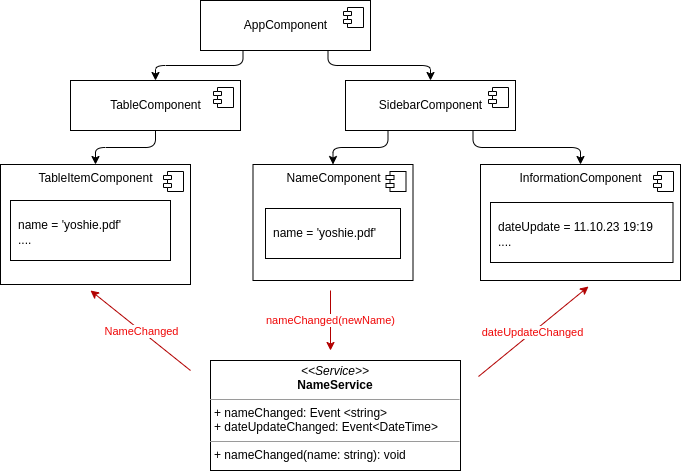
\includegraphics[height=9.5cm]{abbildungen/components-sync-service.png}
\caption{globaler Service: Datenfluss im Komponentenbaum}
\label{components-sync-service}
\end{figure}

Im Beispiel in Abbildung \ref{components-sync-service} wird ein \texttt{NameService} genutzt. Dieser Service bietet eine Methode \texttt{nameChanged}, die von der \texttt{NameComponent} bei Änderungen aufgerufen wird. Die Methode löst dann die Events \texttt{nameChanged} und \texttt{dateUpdateChanged} aus. Haben sich die \texttt{TableItemComponent} und die \texttt{InformationComponent} auf diese Events registriert, werden sie entsprechend benachrichtigt und können ihre angezeigten Werte aktualisieren.

Bei der Entwicklung mit Services bleibt jedoch das Problem der doppelten Datenhaltung bestehen. Im besprochenen Beispiel existiert die Zeichenkette \texttt{name} sowohl in der \texttt{TableItemComponent} als auch in der \texttt{NameComponent}. Dieses Problem lässt sich durch die Verwendung eines zentralen Datenstores auf Basis von Redux umgehen. Dieses Konzept wird im nächsten Abschnitt näher erläutert.


\section{Zentraler Redux-basierter Datenstore}
\label{sec-zentraler-redux-datenstore}

Mit der Zunahme an Komponenten in einer Anwendung steigt auch die Komplexität des zugrundeliegenden Codes. Diese Komplexitätssteigerung resultiert aus der Notwendigkeit, Daten zwischen den Komponenten auszutauschen, um sie in einem konsistenten Zustand zu halten. Zur Reduzierung dieser Komplexität eignet sich der Einsatz eines zentralen, auf Redux basierenden Stores (siehe Abschnitt \ref{sec-komponentenbasierte-webentwicklung}).

\begin{figure}[htbp]
\centering
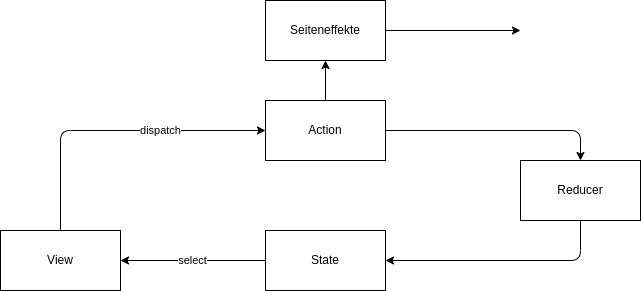
\includegraphics[height=6.5cm]{abbildungen/redux-dataflow.png}
\caption{Von Redux vorgeschriebener Datenfluss}
\label{redux-dataflow}
\end{figure}

Redux, entwickelt von Dan Abramov, ist eine Implementierung des von Facebook definierten Designpatterns Flux. Dieses Pattern sieht einen unidirektionalen Datenfluss vor, wie in Abbildung \ref{redux-dataflow} dargestellt. Der Store verwaltet den gesamten Anwendungszustand bezüglich der darzustellenden Daten. Er bietet Vorteile gegenüber den im vorherigen Abschnitt beschriebenen Konzepten, indem er Datenstrukturen und die gesamte Logik zur Zustandsaktualisierung an einer definierten Stelle konzentriert – bekannt als Single Source of Truth. Zusätzlich verbessert ein zentraler Store nicht nur die Performance, sondern erleichtert auch die Testbarkeit \cite[31-32]{farhi_adding_2017}.

Für eine detaillierte Beschreibung eines Redux-basierten Stores wird auf das bereits verwendete Beispiel zurückgegriffen (siehe auch Abschnitt \ref{sec-komponentenbasierte-webentwicklung}). Dabei wird die Implementierung NgRx \footnote{https://ngrx.io/}, welche im Framework Angular eingesetzt werden kann, verwendet.

\begin{figure}[htbp]
\centering
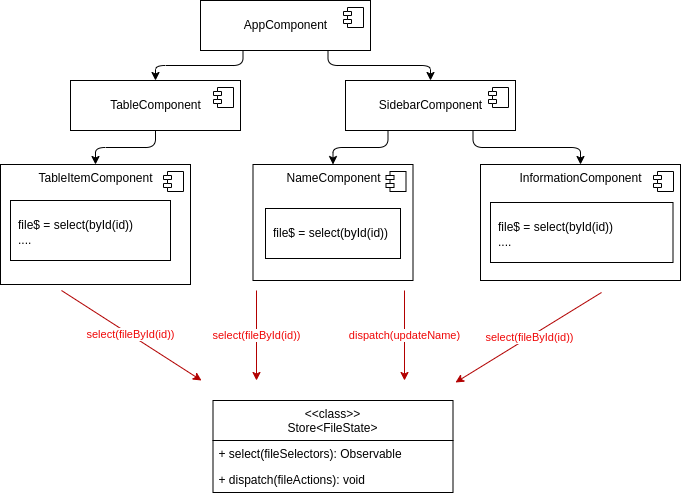
\includegraphics[height=11cm]{abbildungen/easy-state.png}
\caption{Redux-basierter Store: Datenfluss im Komponentenbaum}
\label{redux-easy-state}
\end{figure}

In Abbildung \ref{redux-easy-state} wird illustriert, wie die Komponenten mit dem Store interagieren können, um Daten abzurufen oder Datenänderungen zu veranlassen. Der Store, der wie ein Service global zugänglich ist, bietet zwei Methoden an: Die Methode \texttt{select}, der ein \texttt{Selektor} übergeben wird, steuert, welcher Teil des States zurückgegeben wird. Die Methode gibt kein festes Ergebnis, sondern ein \texttt{Observable} zurück, eine Art Stream. Die Komponente kann sich bei diesem \texttt{Observable} anmelden und wird bei jeder Datenänderung informiert. Um eine Datenänderung zu veranlassen, wird die Methode \texttt{dispatch} verwendet. Dieser wird eine \texttt{Action} übergeben, die definiert, wie die Änderung aussehen soll. Die \texttt{dispatch} Methode gibt keinen Wert zurück, betrifft die gewünschte Änderung jedoch einen Teil des Stores, auf den sich eine Komponente vorab über den Selektor angemeldet hat, wird im gelieferten \texttt{Observable} automatisch ein neuer Wert emittiert.

Im Folgenden werden die Kernkonzepte eines Redux-basierten Stores – der State, die Selektoren, die Actions, der Reducer und die Seiteneffekte – detailliert erläutert.

\subsection{State}
\label{subsec-state}

Der State wird in Form eines einfachen JavaScript-Objekts implementiert und zu Beginn der Anwendung mit vorgegebenen Startwerten initialisiert. Es ist wichtig zu betonen, dass der State ausschließlich lesbar ist; Änderungen am State sind ausschließlich über definierte Reducer-Funktionen möglich, die mittels der \texttt{dispatch}-Funktion aufgerufen werden. Für die Definition des JavaScript-Objekts wird in NgRx ein Interface erstellt, in dem alle benötigten Felder definiert sind. Weiterhin muss eine Konstante definiert werden, die dem Interface entspricht und den initialen Zustand des State festlegt.

\begin{algorithm}
\caption{Statedefinition in NgRx}
\label{alg-stadedefinition-in-ng-rx}
\begin{lstlisting}
export interface FileState {
   entities: {[id: string]: FileObject};
   loaded: boolean;
   loading: boolean;
}

export const initialFileState : FileState = {
    entities: {},
    loaded: false,
    loading: false
}
\end{lstlisting}
\end{algorithm}

Algorithmus \ref{alg-stadedefinition-in-ng-rx} zeigt die Statedefinition für das Beispiel, wie in Abbildung \ref{redux-easy-state} dargestellt. Die beiden Flags \texttt{loaded} und \texttt{loading} geben an, ob die Daten bereits geladen wurden bzw. ob der Ladevorgang bereits gestartet wurde. Die tatsächlichen Daten sind in einem JavaScript-Objekt in Form eines Dictionaries oder einer HashMap abgelegt, wobei die \texttt{id} des \texttt{FileObject} dem Schlüssel und das \texttt{FileObject} selbst dem Wert entspricht. Der Vorteil dieses Ansatzes ist, dass bei bekannter \texttt{id} des \texttt{FileObject} in $O(1)$ auf das Objekt zugegriffen werden kann. Würde man stattdessen ein Array verwenden, müsste bei bekannter \texttt{id} über das gesamte Array iteriert werden, was $O(n)$ Zeit in Anspruch nehmen würde. \cite[54]{bae_javascript_2019}

\subsection{Selektoren}
\label{subsec-selektoren}

Selektoren ermöglichen es Komponenten, auf bestimmte Bereiche des States zuzugreifen. NgRx bietet hierfür die Methoden \texttt{createFeatureSelector} und \texttt{createSelector} an. Die erstere Methode erzeugt einen Selektor, der den gesamten State umfasst. Dafür muss der Methode ein String übergeben werden, der mit dem State-Namen übereinstimmt, der in der Reducer-Definition (siehe \ref{subsec-reducer}) vergeben wird. Die zweite Methode, \texttt{createSelector}, dient dazu, einen Teil des States zu extrahieren, um so kleinere Teile nach außen zu geben.

\begin{algorithm}
\caption{Selektorendefinition in NgRx}
\label{alg-selektorendefinition-in-ng-rx}
\begin{lstlisting}
const state = createFeatureSelector<FileState>('files');
const loaded = createSelector(state, (state) => state.loaded);
const loading = createSelector(state, (state) => state.loading);
const entities = createSelector(state, (state) => state.entities);
//entities as array
const files = createSelector(entities, (entities) => 
    Object.keys(entities).map((id) => entities[id]));
const fileById = (id: string) =>  
    createSelector(entities, (entities) => entities[id]);

export const fileSelectors = {
    loaded, loading, files, fileById
};
\end{lstlisting}
\end{algorithm}

Algorithmus \ref{alg-selektorendefinition-in-ng-rx} zeigt die Selektorendefinition, um auf die für das Beispiel benötigten Teile des States zuzugreifen. Auf die eigentliche Generierung der bereits erwähnten \texttt{Observables} wird in Abschnitt \ref{subsec-facade} näher eingegangen.

\subsection{Actions}
\label{subsec-actions}

Actions in NgRx bestehen aus einer eindeutigen ID und einem optionalen Payload. Zum Erstellen von Actions bietet NgRx die Methode \texttt{createActionGroup()} an, die es ermöglicht, spezifische Actions zu definieren. Die ID einer Action wird aus dem Property-Namen des Events und dem String, der als \texttt{source} angegeben wird, generiert. Die Methoden \texttt{emptyProps()} und \texttt{props()} werden verwendet, um den Payload der Action zu spezifizieren. Algorithmus \ref{alg-actiondefinition-in-ng-rx} zeigt die für das Beispiel notwendigen Action-Definitionen. Die definierten Actions können entweder von außen (siehe Abschnitt \ref{subsec-facade}) oder durch einen Seiteneffekt (siehe Abschnitt \ref{subsec-seiteneffekte}) dispatched werden. Dieses Dispatchen führt in der Regel dazu, dass eine Reducer-Funktion aufgerufen wird, die einen neuen State liefert.

\begin{algorithm}
\caption{Actiondefinitionen in NgRx}
\label{alg-actiondefinition-in-ng-rx}
\begin{lstlisting}
export const fileActions = createActionGroup({
    source: 'files',
    events: {
        load: emptyprops(),
        loadSuccess: props<{files: FileObject[]}>,
        updateName: props<{id: string, name: string}>,
        updateNameSuccess: props<{id: string, name: string}>
    }
})
\end{lstlisting}
\end{algorithm}

\subsection{Reducer}
\label{subsec-reducer}

Über den Reducer wird festgelegt, wie der Store modifiziert werden soll, wenn eine Action ausgeführt (dispatched) wird. Dabei wird für jede Action, die eine Datenänderung bewirken soll, eine sogenannte reine Funktion (pure function) definiert. Dies sind Funktionen, die bei gleichen Eingabeparametern stets dasselbe Ergebnis liefern. Die Parameterwerte der Funktion umfassen den aktuellen State und die ausgeführte Action, wobei der State unverändert bleiben muss (Immutability) \cite[21]{mcfarlane_managing_2019}.


\begin{algorithm}
\caption{Reducerdefinitionen in NgRx}
\label{alg-reducerdefinition-in-ng-rx}
\begin{lstlisting}
const onLoad = (state, action) => 
    ({ loading: true, loaded: false, entities: {} });    
const onLoadSuccess = (state, action) => {
    const entities = arrayToEntities(action.files);
    return { loading: false, loaded: true, entities };
}
const onUpdateNameSuccess = (state, action) => {
    return { ...state, entities: { ...state.entities, 
                [action.id]: {
                    ...state.entities[action.id],
                    name: action.name }
            }}; 
}

export const fileFeature = createFeature({
    name: 'files',
    reducer: createReducer(
        initialFileState,
        on(fileActions.load,onLoad),
        on(fileActions.loadSuccess, onLoadSuccess),
        on(fileActions.updateNameSuccess, onUpdateNameSuccess)
    )})
\end{lstlisting}
\end{algorithm}

Algorithmus \ref{alg-reducerdefinition-in-ng-rx} zeigt die Reducerdefinition in NgRx für das gewohnte Beispiel. Dabei wird ein sogenanntes Feature definiert, dessen \texttt{name} dem String entsprechen muss, der beim Erzeugen des Hauptselektors (der den gesamten State umfasst) verwendet wurde. Die Reducer-Funktionen werden über die Methode \texttt{createReducer} erzeugt. Der erste Parameter muss dabei dem initialen FileState entsprechen (siehe Abschnitt \ref{subsec-state}). Danach wird mittels der Methode \texttt{on} bestimmt, welche Funktion bei welcher Action aufgerufen wird. Wichtig dabei ist zu beachten, dass die Eingabewerte nicht modifiziert werden dürfen, das heißt, es muss, wie in der Methode \texttt{onUpdateNameSuccess} ersichtlich, ein neues State-Objekt retourniert werden.


\subsection{Seiteneffekte}
\label{subsec-seiteneffekte}
Seiteneffekte werden in einem Redux-basierten Store für die Verwaltung von asynchronen Operationen wie API-Aufrufen, Datenpersistenz oder komplexeren Geschäftslogiken verwendet. Sie ermöglichen es, auf bestimmte Actions zu reagieren, ohne den Store direkt zu manipulieren. Diese Operationsweise ist besonders nützlich, wenn externe Prozesse oder asynchrone Aktivitäten involviert sind. In NgRx werden Seiteneffekte mit der \texttt{createEffect}-Funktion definiert, die es ermöglicht, auf spezifische Actions zu reagieren und daraus resultierende Aktionen zu steuern. Im Normalfall wird nach Abschluß der durch die eingehende Action ausgelöste Operation eine ausgehende Action retourniert.

Im Beispiel, das in Algorithmus \ref{alg-seiteneffektsdefinition-in-ng-rx} dargestellt ist, wird auf die Actions \texttt{load} und \texttt{updateName} reagiert. Die Klasse \texttt{FileEffects} wird mit einem Stream aller eintreffenden Actions (\texttt{actions}) initialisiert. Dieser Stream wird verwendet, um auf eingehende Actions zu reagieren. Beispielsweise, wenn die Action \texttt{updateName} eintrifft, löst dies einen API-Aufruf über den \texttt{FileHttpService} aus. Bei erfolgreicher Ausführung des Serveraufrufs wird eine weitere Action, in diesem Fall \texttt{updateNameSuccess}, dispatched.

\begin{algorithm}
\caption{Seiteneffektsdefinitionen in NgRx}
\label{alg-seiteneffektsdefinition-in-ng-rx}
\begin{lstlisting}
@Injectable()
export class FileEffects {
    constructor(actions: Actions, http: FileHttpService) {}

    load$ = createEffect(() => 
        this.actions.pipe(
            ofType(fileActions.load),
            switchMap(() => 
                this.http.load().map((files) => 
                    fileActions.loadSuccess(files))
        ));

    updateName$ = createEffect(() => 
        this.actions.pipe(
            ofType(fileActions.load),
            switchMap(({id, name}) => 
                this.http.updateName(id, name).map(() => 
                    fileActions.updateNameSuccess(id, name))
        ));
}
\end{lstlisting}
\end{algorithm}

\subsection{Fassade}
\label{subsec-facade}

Um die Nutzung des Stores für Komponenten zu vereinfachen und eine lose Kopplung zwischen den Komponenten und den Stores zu erreichen, empfiehlt es sich, eine Fassade zwischen diesen einzuziehen. Eine Fassade fungiert als Abstraktionsschicht, die den Store, die Selektoren und die Actions verbirgt. Dadurch werden öffentliche Methoden nach außen angeboten, sodass die Komponenten keine direkte Kenntnis vom eigentlichen Store haben müssen \cite[266]{freeman_entwurfsmuster_2021}. Algorithmus \ref{alg-facade-beispielimplementierung} zeigt eine Implementierung einer solchen Fassadenklasse, wie sie für das Beispiel benötigt wird.

\begin{algorithm}
\caption{Fassade: Beispielimplementierung für den FileStore}
\label{alg-facade-beispielimplementierung}
\begin{lstlisting}
export class FileFacade {
    constructor(private store: Store<FileState>) {}

    async load() : Promise<boolean> {
        const loaded = await this.store.select(
            fileSelectors.loaded).toPromise();
        if(loaded) return true; //bereits geladen
        
        store.dispatch(fileActions.load()); //ladevorgang starten
        return await this.store.select(
            fileSelectors.loading).pipe(filter(x=>!x))
            .toPromise(); //warten bis Ladevorgang abgeschlossen
    }

    selectAll(): Observable<FileObject[]> =>
        this.store.select(fileSelectors.files());
        
    selectById(id: string): Observable<FileObject> =>
        this.store.select(fileSelectors.fileById(id));

    updateName(id: string, name: string): void =>
        this.store.dispatch(fileActions.updateName({id, name}));
}
\end{lstlisting}
\end{algorithm}

Abbildung \ref{fielStore-dependencies} fasst die Abhängigkeiten zwischen den einzelnen Store-Komponenten zusammen und zeigt, wie durch die Fassade eine lose Kopplung zwischen Store und Komponente erreicht wird.

\begin{figure}[htbp]
\centering
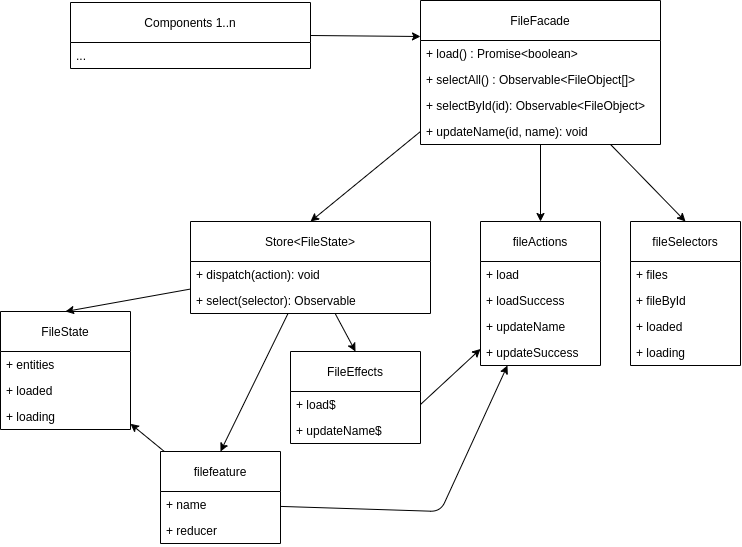
\includegraphics[height=10cm]{abbildungen/easy-state-comp.png}
\caption{FileStore Abhängigkeiten}
\label{fielStore-dependencies}
\end{figure}

\section{WebSocket-Kommunikation}
\label{sec-web-socket-kommunikation}

Wie bereits in Abschnitt \ref{subsec-datenkonsistenz-am-selben-client} erwähnt, besteht in Webanwendungen, insbesondere wenn sie kollaborativ genutzt werden, das Problem, dass bei Datenänderungen alle Clients, die diese Daten geladen haben, aktualisiert werden müssen. Die standardmäßige HTTP-Kommunikation zwischen einem Webclient und dem Server ist zustandslos und kann nur vom Client initiiert werden. Aus der Zustandslosigkeit des HTTP-Protokolls folgt, dass der Server keine Informationen darüber hat, welche Clients gerade verbunden sind und welche Daten diese geladen haben. Um dieses Problem zu lösen, gibt es verschiedene Ansätze wie Long Polling oder WebSockets \cite[182]{ackermann_webentwicklung_2021}. Da \textit{YReduxSocket} von einer WebSocket-Verbindung ausgeht, wird im Folgenden ausschließlich auf dieses Protokoll eingegangen.

Das WebSocket-Protokoll baut auf TCP auf und ermöglicht bidirektionale Verbindungen zwischen Clients und einem Server. Der initiale Verbindungsaufbau muss vom Client ausgehen, doch sobald die Verbindung besteht, hat auch der Server die Möglichkeit, Daten an den Client zu senden \cite[184-185]{ackermann_webentwicklung_2021}. Es kann erforderlich sein, dass sich der Client für relevante Informationen anmeldet, um zu vermeiden, dass der Server bei jeder Datenänderung einen Broadcast (Nachricht an alle verbundenen Clients) senden muss. In Abbildung \ref{easy-websocket-communication} werden zwei Clients dargestellt, die über das WebSocket-Protokoll verbunden sind. Client A führt eine Aktion aus, die Daten ändert. Nach der erfolgreichen Änderung können beide Clients vom Server aus aktualisiert werden.

\begin{figure}[htbp]
\centering
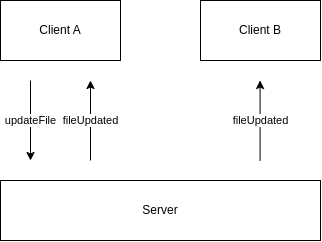
\includegraphics[height=5cm]{abbildungen/websocket-2-clients.png}
\caption{einfache WebSocket Kommunikation}
\label{easy-websocket-communication}
\end{figure}


\section{Datenstore mit WebSocket: herkömmlicher Ansatz}
\label{sec-datenstore-mit-websocket-herkoemmlicher-ansatz}

In der Praxis werden oft beide der oben beschriebenen Technologien gemeinsam eingesetzt. Wenn nun eine WebSocket-Nachricht vom Server gesendet wird, führt dies normalerweise dazu, dass am Client eine entsprechende Aktion ausgelöst wird, die den zentralen Store aktualisiert. Jede neue WebSocket-Nachricht erfordert somit auch die Erstellung einer eigenen Client-Methode, in der auf die Nachricht reagiert und der Store entsprechend angepasst wird. Dadurch ist es nötig, pro WebSocket-Nachricht sowohl server- als auch clientseitige Logik zu implementieren.\\

Wenn nun beispielsweise eine Datenänderung veranlasst wird, die auch anderen Clients angezeigt werden soll, kann wie folgt vorgegangen werden: Der Client, der die Datenänderung auslöst, sendet eine Action an den Datenstore. Im Store ist ein Seiteneffekt definiert, der dazu führt, dass eine HTTP- oder WebSocket-Nachricht an den Server gesendet wird. Der Server verarbeitet den eingehenden Request, indem er beispielsweise Validierungen oder Datenbankänderungen durchführt. Danach sendet der Server eine WebSocket-Nachricht an alle Clients, die sich zuvor für Benachrichtigungen angemeldet haben. Die Clients empfangen die WebSocket-Nachricht und verarbeiten sie, indem sie eine weitere Action an den Store senden. Diese Action aktiviert den Reducer, der den Datenstore anpasst. Bei der Implementierung neuer Funktionen, die eine Server-Client-WebSocket-Kommunikation erfordern, muss der Entwickler die folgenden Schritte durchführen:
\begin{enumerate}
    \item Definition einer Action, die den Seiteneffekt auslöst.
    \item Definition einer Action, die für eine Anpassung durch den Reducer sorgt.
    \item Implementierung eines neuen WebSocket-Endpunkts auf der Serverseite.
    \item Implementierung des Seiteneffekts, der den WebSocket-Endpunkt aufruft.
    \item Implementierung der serverseitigen Validierungs- und Anpassungslogik.
    \item Implementierung eines neuen WebSocket-Endpunkts auf der Clientseite. Dieser sendet die Reducer-Action an den Store.
    \item Aufruf des Client-Endpunkts auf der Serverseite.
    \item Implementierung der Reducer-Funktion, die die eigentlichen Client-Daten anpasst.
\end{enumerate}

%--------------STAND DER TECHNIK--------------
%--------------------------------------
\chapter{Stand der Technik}
\label{chap-stand-der-technik}

\section{Verwandte Arbeiten}
\label{sec-verwandte-arbeiten}

In einer Arbeit von Qu et al. \cite{qu_websocket-based_2019} wird ein Entwicklungsframework vorgestellt, das die WebSocket-Technologie mit einem Redux-basierten Datenstore verknüpft. Diese Arbeit konzentriert sich jedoch ausschließlich auf die Verwendung der JavaScript-Frameworks React auf der Clientseite und Node.js auf der Serverseite. Im Gegensatz dazu ist das Ziel dieser Arbeit die Entwicklung einer generischen Spezifikation, die unabhängig von den eingesetzten Frameworks implementiert werden kann. \\

Weitere verwandte Arbeiten, wie die von McFarlane \cite{mcfarlane_managing_2019} oder Tuomi \cite{tuomi_automated_2018}, behandeln oder erwähnen ebenfalls das Thema, beschränken sich jedoch ebenfalls auf die Verwendung der Frameworks React oder Node.js. \\

Die oben genannten Arbeiten werden voraussichtlich in die im Kapitel \ref{chap-y-redux-socket} beschriebenen Vergleiche einbezogen, um einen umfassenden Überblick über die Leistungsfähigkeit und Anwendbarkeit der entwickelten Lösung zu erhalten.

\section{Analyse der verwandten Arbeiten}
\label{analyse-der-verwandten-arbeiten}

%--------------YReduxSocket-------
%---------------------------------
\chapter{YReduxSocket}
\label{chap-y-redux-socket}

\section{Generische Konzeption und Spezifikation}
\label{sec-generische-konzeption-und-spezifikation}

Die Idee hinter YReduxSocket ist nun den in Abschnitt \ref{sec-datenstore-mit-websocket-herkoemmlicher-ansatz} beschriebenen Ansatz zu vereinfachen. Dabei werden die Actions sowohl auf der Server als auch auf der Clientseite definiert. Anstatt die Action nun an den Store zu senden, wird sie direkt an den Server übermittelt. Der Server benötigt lediglich einen einzigen WebSocket- oder HTTP-Endpunkt zum Empfangen der Action. Dieser Endpunkt führt dazu, dass eine Methode ausgeführt wird, in der je nach Identifikationszeichenfolge der Action entschieden wird, welche Validierungen oder Datenbankänderungen durchgeführt werden sollen. Nach Abschluss sendet der Server wieder eine Action per WebSocket an den Client. Dies geschieht ebenfalls über eine zuvor bereits definierte Client-Methode. In dieser Methode muss der Client lediglich sicherstellen, dass die Action an den Store weitergeleitet wird. Über die weitergeleitete Action wird dann der Reducer aktiviert, der den Store anpasst. Wenn neue Endpunkte benötigt werden, kann auf Seiteneffekte, die die Server-Client-Kommunikation behandeln, vollständig verzichtet werden. Mit dieser Idee muss eine Entwicklerin die folgenden Schritte durchführen, um die Server-Client-Kommunikation zu erweitern:
\begin{enumerate}
    \item Definition von zwei Actions auf der Client- und der Serverseite.
    \item Senden einer Action an den Server durch Aufruf des vorhandenen Endpunkts.
    \item Implementierung der serverseitigen Validierungs- und Anpassungslogik.
    \item Aufruf des vorhandenen Client-Endpunkts auf der Serverseite, wobei die zweite Action übergeben wird.
    \item Implementierung der Reducer-Funktion, die die eigentlichen Client-Daten anpasst.
\end{enumerate}

Ein Vergleich mit den Umsetzungsschritten aus Abschnitt \ref{sec-datenstore-mit-websocket-herkoemmlicher-ansatz} egibt, dass der vorgestellte Ansatz erheblich weniger Implementierungsaufwand erfordert.

\section{Konsistenzverhalten}
\label{sec-konsistenzverhalten}

Durch den Einsatz eines Redux-basierten Datenstores verfügt jeder beteiligte Client über seine eigene "`Single Source of Truth"'. Es ist jedoch wichtig zu beachten, dass die tatsächliche Wahrheit in der von einem Server verwalteten Datenbank liegt. Hier können bei Lese-Schreib- oder Schreib-Schreib-Konflikten sowie bei kurzzeitigen Unterbrechungen der WebSocket-Verbindung Inkonsistenzen zwischen den einzelnen Stores der Clients auftreten. Das JavaScript-Objekt welches vom Datenstore verwendet wird existiert im RAM des Webbrowsers, was bedeutet, dass beim Neuladen der Anwendung die Daten erneut vom Server abgerufen werden und der Datenstore wieder dem Zustand der Datenbank entspricht. Darüber hinaus werden die Daten aktualisiert, wenn eine neue Erfolgsmeldung eines Aktualisierungsvorgangs eintrifft. In diesem Kontext kann laut Tannenbaum und Van Steen von "`eventual consistency"' gesprochen werden \cite[319, 322]{tanenbaum_verteilte_2008}. \\ 

Für viele Anwendungsfälle ist diese "`eventual consistency"' durchaus ausreichend. Es gibt jedoch Szenarien, in denen eine hohe Konsistenz zwischen den einzelnen Clients bzw. Client-Stores erforderlich ist. Dabei wurde ein Algorithmus von Marijn Haverbeke verwendet \cite{haverbeke_collaborative_2015}, der in YReduxSocket implementiert wurde. Vereinfacht funktioniert der Algorithmus folgendermaßen:

\begin{itemize}
    \item Am Server werden die Actions (beispielsweise über eine Redis-Datenbank) an zentraler Stelle gesammelt.
    \item Alle Actions desselben Typs haben eine Versionsnummer.
    \item Auch die Clients haben die zuletzt gesendete Versionsnummer gespeichert.
    \item Wenn ein Client eine neue Action auslösen möchte, sendet er sie zusammen mit seiner Versionsnummer an den Server.
\end{itemize}

Nun unterscheidet der Algorithmus 2 Fälle. \\

\textbf{Die Versionsnummer des Clients stimmt mit der des Servers überein:}

\begin{itemize}
    \item Wenn die Versionsnummer am Server mit der des Clients übereinstimmt, wird die Action ausgeführt (Datenbankanpassung) und im Redis-Cache gespeichert.
    \item Darüber hinaus werden alle anderen Clients, die sich für diese Action angemeldet haben, über eine "NewAction"-Meldung benachrichtigt.
    \item Anschließend erhöhen alle Clients ihre Versionsnummer.
\end{itemize}

\textbf{Die Versionsnummer des Clients stimmt nicht mit der des Servers überein:}

\begin{itemize}
    \item In diesem Fall verwirft der Server einfach die empfangene Action.
    \item Da die Versionsnummern nicht übereinstimmen, wurde eine "`NewAction"'-Meldung an den ausführenden Client gesendet.
    \item Wenn die "`NewAction"'-Meldung eintrifft, holt sich der Client alle Actions, die größer sind als seine eigene Versionsnummer, vom Server und wendet sie auf seinem Redux-Store an.
    \item Danach sendet er seinen Änderungswunsch (Action) erneut an den Server.
\end{itemize}

Es ist erwähnenswert, dass das Konsistenzproblem nicht nur bei YReduxSocket, sondern auch im herkömmlichen Modell auftritt.

\subsection{eventual consistency}
\label{subsec-eventual-consistency}

\subsection{Algorithmus von H.}
\label{subsec-algorithmus-von-h}

\subsection{Alternative Ansätze}
\label{subsec-alternative-ansaetze}
\begin{itemize}
    \item Vektoruhren?
\end{itemize}

\section{Vergleich mit herkömmlichen Ansatz}
\label{sec-vergleich-mit-herkoemmlichen-ansatz}

\section{Vergleich mit verwandten Arbeiten}
\label{sec-vergleich-mit-verwandten-arbeiten}


%--------------Implementierung und Tests-------
%----------------------------------------------
\chapter{Implementierung und Tests}
\label{chap-implementierung-und-tests}

\section{Angular und ASP.NET}
\label{sec-angular-und-aps-net}

\section{React und Node.js}
\label{sec-react-und-node-js}

\section{npm und NuGet}
\label{sec-npm-und-nu-get}

%--------------Fazit-------
%--------------------------
\chapter{Fazit}
\label{chap-fazit}

\section{Zusammenfassung}
\label{sec-zusammenfassung}

\section{Validierung der Lösung}
\label{sec-validierung-der-loesung}

\section{Potenzielle Verbesserungen des Konzepts}
\label{sec-potenzielle-verbesserungen-des-konzepts}

\printbibliography

\appendix

\chapter{Eigenständigkeitserklärung}

\enquote{Ich erkläre, dass ich die schriftliche Ausarbeitung zur Abschlussarbeit selbstständig und ohne unzulässige Inanspruchnahme Dritter verfasst habe. Ich habe dabei nur die angegebenen Quellen und Hilfsmittel verwendet und die aus diesen wörtlich oder sinngemäß entnommenen Stellen als solche kenntlich gemacht. 
Die Versicherung selbstständiger Arbeit gilt auch für enthaltene Zeichnungen, Skizzen oder graphische Darstellungen. Die Ausarbeitung wurde bisher in gleicher oder ähnlicher Form weder derselben noch einer anderen Prüfungsbehörde vorgelegt und auch nicht veröffentlicht. 
Mit der Abgabe der elektronischen Fassung der endgültigen Version der Ausarbeitung nehme ich zur Kenntnis, dass diese mit Hilfe eines Plagiatserkennungsdienstes auf enthaltene Plagiate geprüft werden kann und ausschließlich für Prüfungszwecke gespeichert wird.}\\\\\\

\begin{tabular}{@{}l@{}}\hline
Ricardo Stolzlechner
\end{tabular}\\\\\\

\end{document}
